% Copyright (c) 2022 Tobias Briones. All rights reserved.
% SPDX-License-Identifier: CC-BY-SA-4.0
%
% This source code is part of
% https://github.com/tobiasbriones/cp-unah-is911-microprocessors and is
% licensed under the Creative Commons Attribution Share Alike 4.0
% International License found in the LICENSE file in the root
% directory of this source tree or at https://spdx.org/licenses/CC-BY-SA-4.0

\documentclass{article}
\usepackage{preamble}

\title{LAB 4: RASPBERRY PI PICO Y MICROPYTHON}
\author{Tobias Briones \bigbreak tobias.briones@unah.hn}
\date{\today}

\begin{document}

    \makeatletter
    \begin{titlepage}
        \begin{center}
            
\includegraphics[width=0.3\linewidth]{images/logo-unah}\\[4ex]
            {\huge \bfseries \@title
            \vspace{1cm}}\\[2ex]
            {\LARGE \@author}\\[50ex]

            {\large
            Universidad Nacional Autónoma de Honduras\\
            Ingeniería de Sistemas\\
            I PAC 2022\\
            IS911-MICROPROCESADORES
            }\\[2ex]

            {\large \today}
        \end{center}
    \end{titlepage}
    \makeatother
    \thispagestyle{empty}
    \newpage

    \import{}{footer}

    \section{Objetivo}

    Desarrollar ejemplos de programas básicos para simular en Raspberry Pi Pico y MicroPython.


    \subsection{Objetivos Específicos}\label{subsec:objetivos-específicos}

    \begin{itemize}
        \item Utilizar un simulador en línea que permita hacer los proyectos.
        \item Entender la tarjeta Raspberry Pi Pico tanto en programación como en circuito.
        \item Desarrollar $3$ ejercicios prácticos en total.
    \end{itemize}

    \section{Marco Teórico}\label{sec:marco-teórico}



    \section{Procedimiento Experimental}\label{sec:procedimiento-experimental}

    Para hacer los experimentos se usa \href{https://wokwi.com}{Wokwi}. En este se desarrollará el programa como el circuito y su simulación para cada ejercicio.

    \subsection{Ejemplo 1}

    Desarrollar un programa en MicroPython para Raspberry Pi Pico que encienda un LED cuando se mantenga presionado un botón.

    \bigbreak

    \textit{Solución:}

    \bigbreak

    El programa que se necesitará es sencillo:

    \begin{lstlisting}[language=Python, caption={Programa para el ejemplo 1}]
    import machine

    led = machine.Pin(18, machine.Pin.OUT)
    button = machine.Pin(0, machine.Pin.IN)

    while True:
        led.value(1) if button.value() == 1 else led.value(0)
    \end{lstlisting}

    Similar a como se programa en Arduino, primero se crearon dos variables para manejar la salida en el pin $18$ del LED y así también la entrada del pulsador en el pin $0$.

    \bigbreak

    Así, se puede construir el loop del programa el cual corre indefinidamente para ejecutar la lógica de programación. En este caso se define el valor ($1$ o $0$) del LED dependiendo del valor del pulsador en la entrada.

    \bigbreak

    El circuito se desarrollará de la siguiente manera:

    \begin{figure}[H]
        \centering
        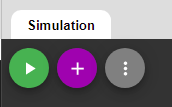
\includegraphics[width=0.2\paperwidth]{images/wokwi-actions}
        \caption{Acciones disponibles en el menú de Wokwi}
    \end{figure}

    En la acción \say{Add a new part} se puede seleccionar un dispositivo para agregar al circuito.

    \begin{figure}[H]
        \centering
        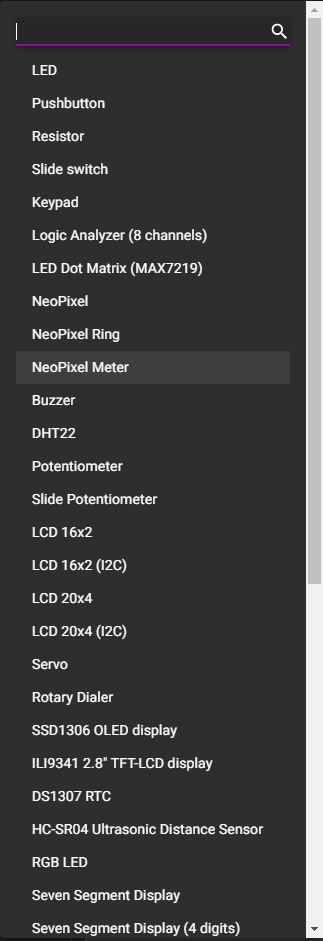
\includegraphics[width=0.2\paperwidth]{images/wokwi-parts}
        \caption{Partes o dispositivos en Wokwi}
    \end{figure}

    De esa forma, se puede agregar cualquier dispositivo como LED, resistencia, etc., a fin de elaborar el circuito. El circuito de este ejemplo es como sigue:

    \begin{figure}[H]
        \centering
        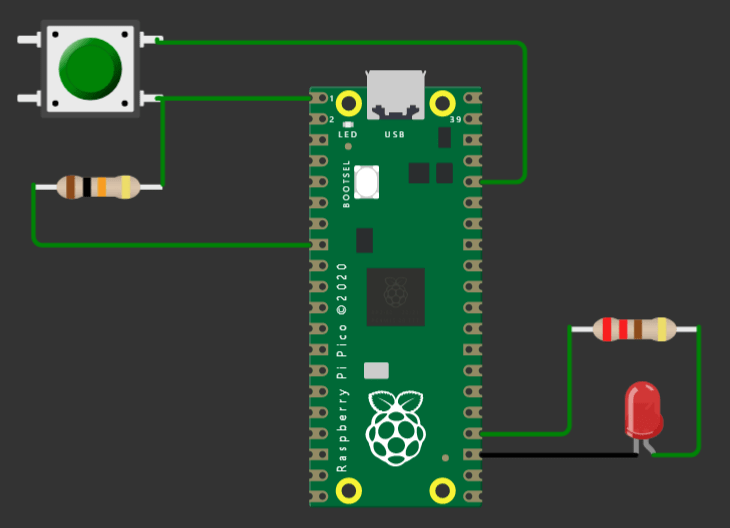
\includegraphics[width=0.4\paperwidth]{images/wokwi-example-1-circuit}
        \caption{Circuito para el ejemplo 1}
    \end{figure}

    Notar que al hacer hover en un pin se muestra mayor información sobre ese pin. La conexión a tierra se hace simplemente con uno de los pines tierra de la tarjeta.

    \bigbreak

    Por último, hay una pestaña para configurar los atributos de los dispositivos que se han agregado al proyecto. Se puede modificar el valor de la resistencia así como cualquier atributo de cada parte o dispositivo.

    \begin{figure}[H]
        \centering
        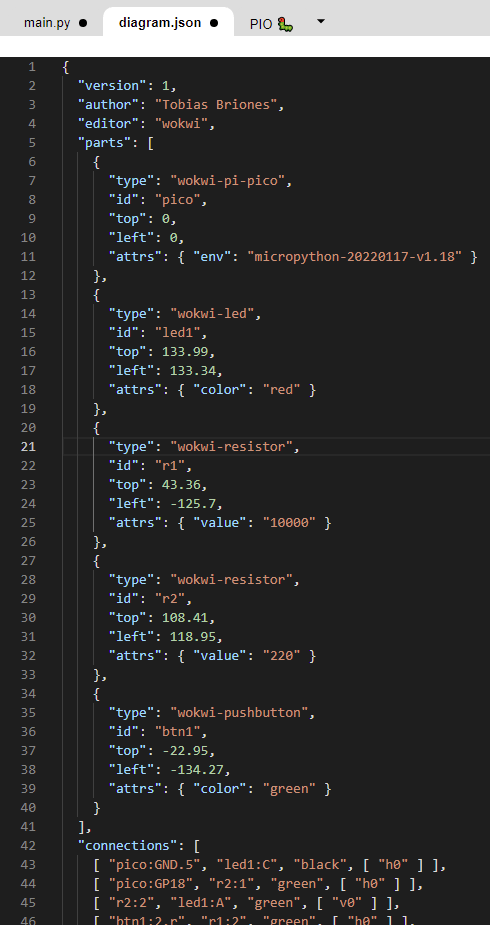
\includegraphics[width=0.3\paperwidth]{images/wokwi-example-1-diagram-src-code}
        \caption{Código fuente del circuito}
    \end{figure}

    \subsection{Ejemplo 2}

    Desarrollar un programa que tome dos entradas $A$ y $B$ y tenga dos salidas $Z_1$ y $Z_2$ que computen la compuerta lógica $AND$ y $OR$ de las entradas respectivamente.

    \bigbreak

    \textit{Solución:}

    \bigbreak

    De la misma manera que se desarrolló el ejemplo anterior, se seguirán trabajando los restantes. Por tanto, tenemos el código y circuito para este ejemplo:

    \begin{lstlisting}[language=Python, caption={Programa para el ejemplo 2}]
    import machine

    A = machine.Pin(1, machine.Pin.IN)
    B = machine.Pin(2, machine.Pin.IN)
    Z0 = machine.Pin(12, machine.Pin.OUT)
    Z1 = machine.Pin(13, machine.Pin.OUT)

    while True:
        Z0.value(A.value() and B.value())
        Z1.value(A.value() or B.value())
    \end{lstlisting}

    Se crean las entradas y las salidas, y en el loop se calculan los valores lógicos para asignar a la salida.

    \begin{figure}[H]
        \centering
        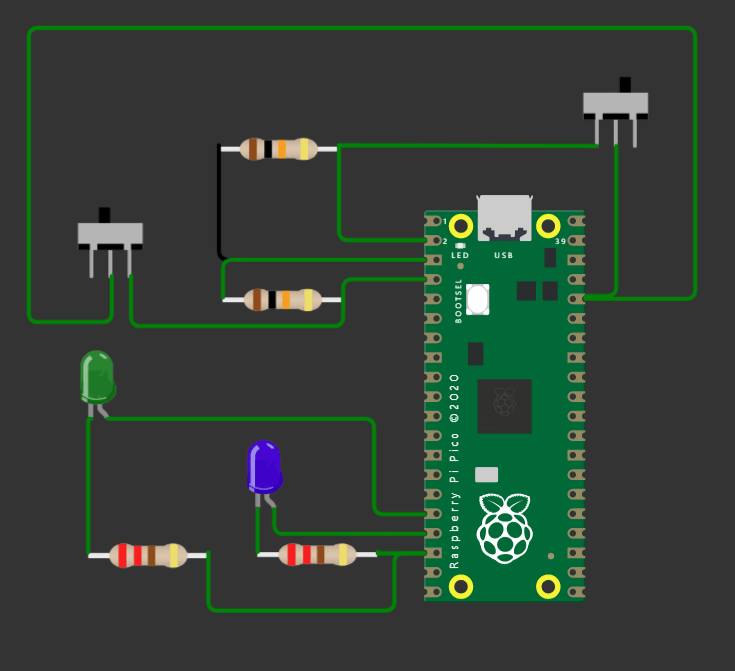
\includegraphics[width=0.5\paperwidth]{images/wokwi-example-2-circuit}
        \caption{Circuito para el ejemplo 2}
    \end{figure}

    \begin{figure}[H]
        \centering
        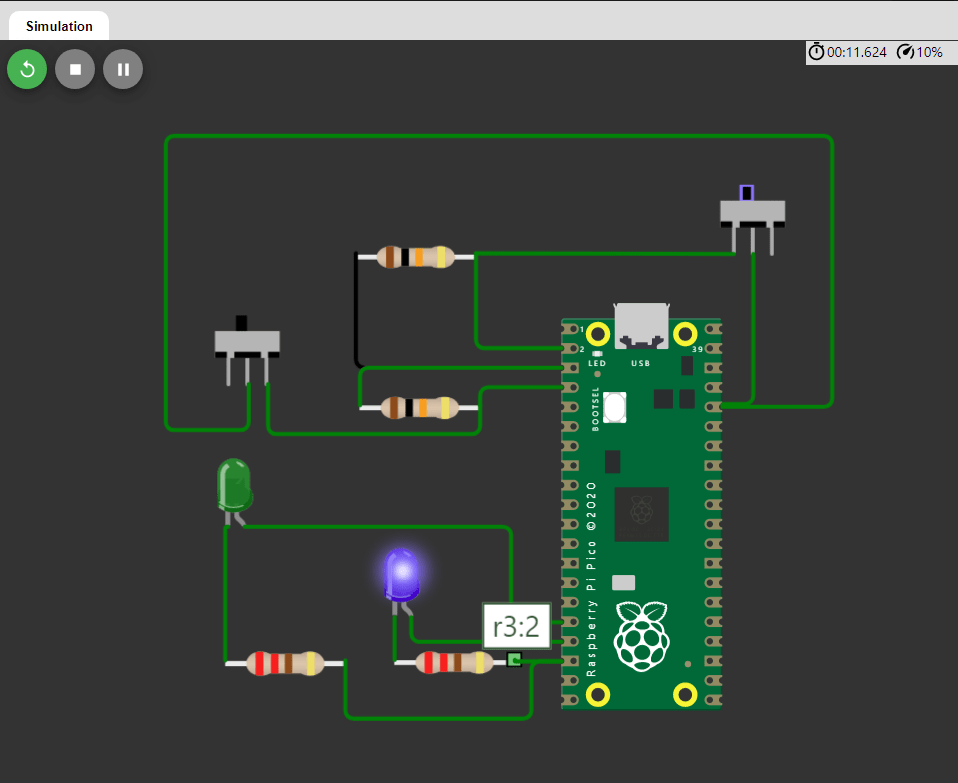
\includegraphics[width=0.5\paperwidth]{images/wokwi-example-2-sim-1}
        \caption{Simulación 1 (OR)}
    \end{figure}

    \begin{figure}[H]
        \centering
        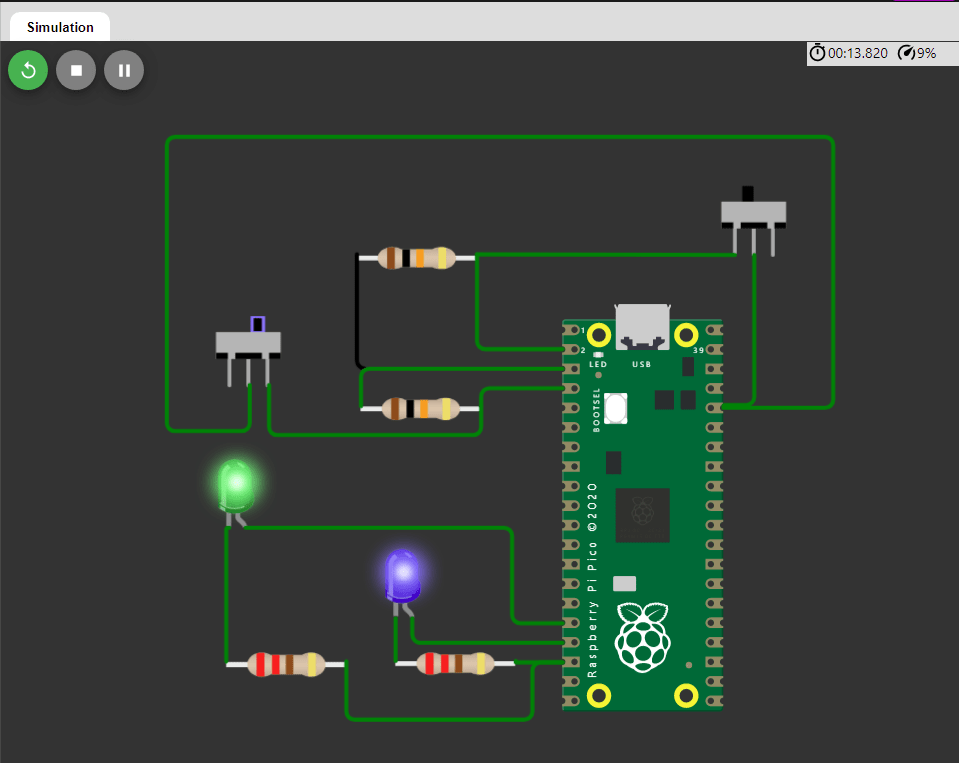
\includegraphics[width=0.5\paperwidth]{images/wokwi-example-2-sim-2}
        \caption{Simulación 2 (AND, OR)}
    \end{figure}

    Como se puede ver en las capturas, al tener uno o dos interruptores cerrados se obtiene un uno lógico en la salida del LED azul y al tener ambos interruptores cerrados ya se activa el LED verde.


    \section{Análisis de Resultados}\label{sec:análisis-de-resultados}



    \section{Conclusión}\label{sec:conclusion}



    \printbibliography

\end{document}
